\documentclass[CJK]{beamer}

\usepackage{CJK}
\usepackage{color}
\usepackage{graphicx}
\usepackage{listings}
\usepackage{xcolor}
\lstset{
  %行号
  %numbers=left,
  %背景框
  %framexleftmargin=10mm,
  %frame=none,
  %背景色
  %backgroundcolor=\color[rgb]{1,1,0.76},
  backgroundcolor=\color[RGB]{245,245,244},
  %样式
  keywordstyle=\bf\color{blue},
  identifierstyle=\bf,
  numberstyle=\color[RGB]{0,192,192},
  commentstyle=\it\color[RGB]{0,96,96},
  stringstyle=\rmfamily\slshape\color[RGB]{128,0,0},
  %显示空格
  showstringspaces=false
}

\hypersetup{CJKbookmarks=true}
\usetheme{PaloAlto}

\begin{document}
\begin{CJK}{UTF8}{gbsn}

\title[Simulator]{\huge Unicore Simulator Interim Report}
\author[Author]{\begin{center}Li Chunqi \and Peng Zhuo \\ Wang Kan \and Hua Liansheng\end{center}}
\date{\today}

\begin{frame}
  \titlepage
\end{frame}

%%%%%%%%%%%%%%%%%%%%%%%%%%%%%%%%%%%
\section*{Contents}

\begin{frame}
  \hypertarget{Contents}
  \frametitle{Contents}
  \tableofcontents[pausesection]
\end{frame}

%%%%%%%%%%%%%%%%%%%%%%%%%%%%%%%%%%
\section{Project Review}

\begin{frame}
  \huge{Project Review}
\end{frame}

\subsection{Project Target Review}
\begin{frame}
  \frametitle{Project Target Review}
  \begin{itemize}
    \item
      Realize CPU controller and datapath with {\color{red}five} level pipline
    \item
      Realize at least one level cache, {\color{red}Havard architecture}.
    \item
      Realize dynamic memory management.
    \item
      Support of some system library functions.
    \item
      Debugger utils and Performance Analysis utils support.
  \end{itemize}
\end{frame}

\subsection{Expected Progress}
\begin{frame}
  \frametitle{Expected Progress}
  \begin{itemize}
    \item
      {\color{blue}1-2 weeks} ELF parser module, Register heap module, Memory module. {\color{red}(Finished in 1st week)}
    \item
      {\color{blue}3-4 weeks} CPU module. {\color{red}(Finished in 4th week)}
    \item
      {\color{blue}5-6 weeks} Cache module{\color{red}(Finished in 3rd week)}, Loader module. {\color{red}(Finished in 2nd week)}
    \item
      {\color{blue}7-8 weeks} Debugger module and some latter works.{\color{red}(To be finished in 1-2 week)}
  \end{itemize}
  More infomation about our project progress, see our svn:

  {\color{blue}http://code.google.com/p/minic/wiki/MINICintroduction?tm=6}
\end{frame}

%%%%%%%%%%%%%%%%%%%%%%%%%%%%%%%%%%
\section{Project Introduction}

\begin{frame}
  \huge{Project Introduction}
\end{frame}

\subsection{Module View}
\begin{frame}
  \frametitle{Module View}
  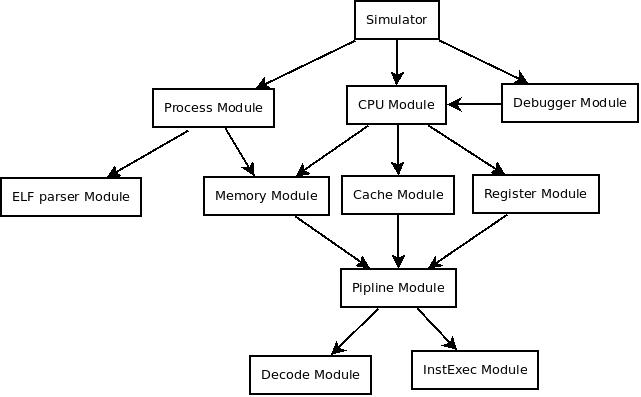
\includegraphics[height=5cm]{module_view.jpeg}
\end{frame}

\subsection{File View}
\begin{frame}
  \frametitle{File View}
Simulator (simulator.c)\\
~~\textbar ------Process Module (process.c)\\
~~\textbar ~~ \textbar ------ELF\_parser Module (ELF\_parser.c)\\
~~\textbar ~~ \textbar ------Memory Module (mem.c)\\
~~\textbar\\
~~\textbar ------CPU Module (CPU.c)\\
~~\textbar ~~ \textbar ------Cache Module (cache.c)\\
~~\textbar ~~ \textbar ------Register Module (register.c)\\
~~\textbar ~~ \textbar ------Pipline Module (pipline.c)\\
~~\textbar ~~ \textbar ~~ \textbar ------Decode Module (decode.c)\\
~~\textbar ~~ \textbar ~~ \textbar ------Instruction Execuation Module (instEx.c)\\
~~\textbar\\
~~\textbar ------Debugger Module (Debugger.c)\\
~~\textbar
\end{frame}

%%%%%%%%%%%%%%%%%%%%%%%%%%%%%%%%%%%%%%%%%
\section{Module Analysis}

\begin{frame}
  \huge{Module Analysis}
\end{frame}

\subsection{Process Module}
\begin{frame}[fragile]
  \frametitle{Process Module}
  Struct of Process:
\begin{lstlisting}[language={C}]
typedef struct{
  int status; //Process status
  uint32_t entry; //The entry of a program
  PROC_STACK* stack; //Process stack
  PROC_MEM* mem; //Process memory
}PROCESS;
\end{lstlisting}
  Process is a basic module handles a copy of a progrss in the memory.
\end{frame}

\subsection{CPU Module}
\begin{frame}[fragile]
  \frametitle{CPU Module}
  CPU Module is the most important module, it lays on the top level and handles add the execuation of a progress.\\
  Struct of CPU:
\begin{lstlisting}[language={C}]
typedef struct{
  int cpu_id; //CPU id
  int mode; //CPU mode, normal or trap
  REGISTERS* regs; //Register heap
  CACHE *i_cache, *d_cache;
  PIPLINE * pipline; //CPU pipline
  PROCESS* proc; //Process running on CPU now
  CPU_info* cpu_info; //Information of CPU
                      //from starting
}CPU_d;
\end{lstlisting}
\end{frame}

\begin{frame}[fragile]
  \frametitle{CPU Module(cont.)}
  Struct of CPU\_info:
\begin{lstlisting}[language={C}]
typedef struct{
  int cycles_total;//total cycles of cpu
  int cycles_work;//work cycles of cpu
  int bubbles;//bubbles of pipline
  int rd_mem_times;//times of read memory
  int wr_mem_times;//times of write memory
  int cache_visit;//times of cache visit
  int cache_miss;//times of cache miss
}CPU_info;
\end{lstlisting}
\end{frame}

\subsection{Memory Module}
\begin{frame}[fragile]
  \frametitle{Memory Module}
  Struct of Process Memory Management:
\begin{lstlisting}[language={C}]
typedef struct{
  unsigned int vaddr_offset;
  unsigned int size;
  uint8_t *base;
  int flag;
}PROC_SEGMENT;

typedef struct{
  unsigned int seg_num;
  PROC_SEGMENT * segments;
}PROC_MEM;

typedef PROC_SEGMENT PROC_STACK;
\end{lstlisting}
\end{frame}

\subsection{Cache and Register Module}
\begin{frame}[fragile]
  \frametitle{Cache and Register Module}
  Struct of Cache and Register Module:
\begin{lstlisting}[language={C}]
typedef struct{
  int block_num;
  int sign_bits_num;
  PROC_MEM* mem;
  int valid[CACHE_SIZE/BLOCK_SIZE];
  uint8_t data[CACHE_SIZE/BLOCK_SIZE][BLOCK_SIZE];
  uint32_t mark[CACHE_SIZE/_BLOCK_SIZE];
}CACHE;

typedef struct{
  int32_t r[32];
  int32_t flag;
}REGISTERS;
\end{lstlisting}
\end{frame}

\subsection{Pipline Module}
\begin{frame}[fragile]
  \frametitle{Pipline Module}
  Struct of Pipline:
\begin{lstlisting}[language={C}]
typedef struct{
  int block;//1 means pipline block, 0 mean the opposite
  PIPLINE_DATA* pipline_data[PIPLINE_LEVEL];
  int using_regs[31];
  PROC_STACK* stack;
  REGISTERS* regs;
  CACHE *i_cache, *d_cache;
}PIPLINE;
\end{lstlisting}
\end{frame}

\begin{frame}
  \frametitle{Total Lines}
  Project has {\color{blue}1987} lines until now.(Exclude blank lines)
  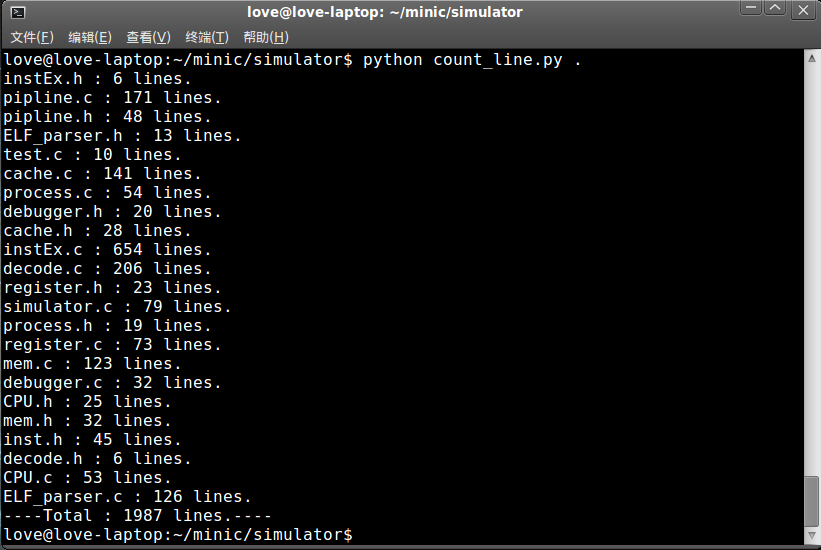
\includegraphics[height=5cm]{count_line.png}
\end{frame}

%%%%%%%%%%%%%%%%%%%%%%%%%%%%%%%%%%%%%%%%%%%%%%
\section{Project Bottleneck}

\begin{frame}
  \huge{Summary Before Mid-term Check}
\end{frame}

\begin{frame}
  \frametitle{Project Bottleneck}
  Some problems when do the project
  \begin{enumerate}
    \item Keeping each module independent is important but difficult.
    \item System library function handling is yet left to be realized.
    \item Some instructions are not realized because of lacking manual.
    \item Instruction execuation module is hard to test and verify, bacause constructing test set is sometimes ambiguous.
    \item Too many modules leads to high maintenance cost.
    \item Some potential bugs need to be resolved.
  \end{enumerate}
\end{frame}

%%%%%%%%%%%%%%%%%%%%%%%%%%%%%%%%%%%%%%%%%%%%%%%
\section{Future Work}

\begin{frame}
  \frametitle{Future Work}
  Future work in next 1-2 weeks:
  \begin{itemize}
    \item Complete Debugger module and high level console.
    \item Finish verification outline.
    \item Construct high-level test set(generate by c files) and low-level test set(generate by assembler files).
    \item Discuss and solve the problem of system library function call.
    \item A complete program compiled by unicore32-linux-gcc(the given compiler from lab) can be run completely in out simulator.
  \end{itemize}
\end{frame}

\begin{frame}
  Q\&A
\end{frame}


\end{CJK}
\end{document}
